\documentclass[tikz,border=2pt]{standalone}
\usepackage{amsmath,amssymb}
\usepackage{tikz}
\usetikzlibrary{arrows.meta}

\begin{document}
% Maximum zero-cost matching as a max flow: source -> rows, row -> column where the reduced
% matrix has a zero, columns -> sink, all capacities 1; the max flow value (2) is the size of
% the largest independent set of zeros.
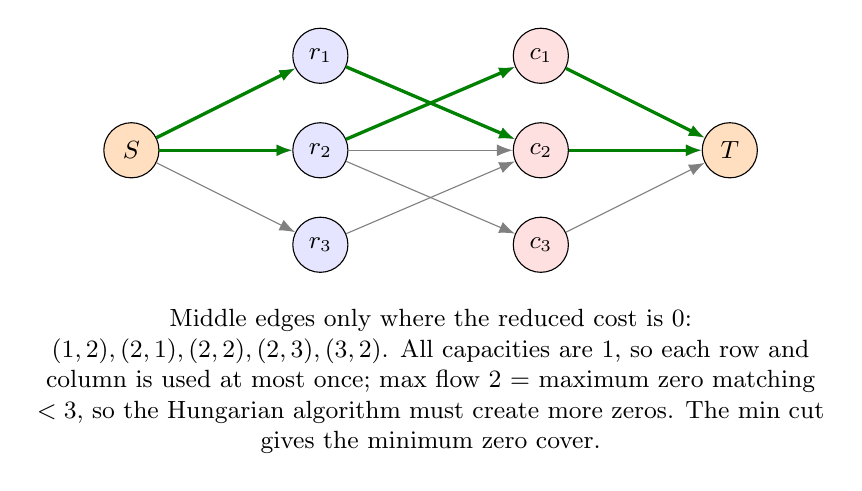
\begin{tikzpicture}[every node/.style={font=\small}, >={Latex[length=2mm]}, v/.style={draw, circle, fill=blue!10, minimum size=7mm, inner sep=0pt}, w/.style={draw, circle, fill=red!12, minimum size=7mm, inner sep=0pt}, st/.style={draw, circle, fill=orange!25, minimum size=7mm, inner sep=0pt}]
	\node[st] (S) at (0,0) {$S$};
	\foreach \i in {1,2,3} {\node[v] (r\i) at (2.4,{2.4-1.2*\i}) {$r_\i$};}
	\foreach \j in {1,2,3} {\node[w] (c\j) at (5.2,{2.4-1.2*\j}) {$c_\j$};}
	\node[st] (T) at (7.6,0) {$T$};
	\foreach \i in {1,2,3} {\draw[->, gray] (S) -- (r\i);}
	\foreach \j in {1,2,3} {\draw[->, gray] (c\j) -- (T);}
	\foreach \i/\j in {1/2, 2/1, 2/2, 2/3, 3/2} {\draw[->, gray] (r\i) -- (c\j);}
	\draw[->, green!50!black, very thick] (S) -- (r1); \draw[->, green!50!black, very thick] (r1) -- (c2); \draw[->, green!50!black, very thick] (c2) -- (T);
	\draw[->, green!50!black, very thick] (S) -- (r2); \draw[->, green!50!black, very thick] (r2) -- (c1); \draw[->, green!50!black, very thick] (c1) -- (T);
	\node[anchor=north, align=flush center, text width=10cm] at (3.8,-1.9) {Middle edges only where the reduced cost is $0$: $(1,2),(2,1),(2,2),(2,3),(3,2)$. All capacities are $1$, so each row and column is used at most once; max flow $2$ $=$ maximum zero matching $<3$, so the Hungarian algorithm must create more zeros. The min cut gives the minimum zero cover.};
\end{tikzpicture}
\end{document}
